%#!platex -kanji=utf8 hb.tex
\chapter{表の構成}% 表組
% これはただのダミーテキスト.
% 文字コードを判定するための意味のない文字列.
% これくらい記述すれば大丈夫かな.
% Emacs のくせに生意気な.
% Emacs の分際で自動判別とか.
% Mac OS X のテキストエディッタの文字コード自動判別はうまくいかないぞ.

\section{表}
\LaTeX で表を作るために三つの環境が用意されています.
\begin{description}
 \item[\Env{tabbing}環境] 
   タブを制御する事によって表を作成する.
 \item[\Env{tabular}環境] 
   高度な表も作成する事ができる汎用的な表作成環境.
 \item[\Env{array}環境]
   \env{tabular}環境と機能は類似しているが数式の
   行列などに使われる事が多い.
\end{description}
\env{array}環境は
\secref{math:array}にて紹介しています
のでそちらを参照してください.\env{tabbing}環境
も簡単に表が作成できる環境なのですが,\env{tabular}
のほうが記述が楽だと思いますので,ここでは\env{tabular}
のみを紹介します.\env{tabular}環境は次のように
記述します.
\begin{usage}
\begin{tabular}[$\<位置指定>$]{$\<列指定>$}
$\begin{array}{*6c}\text{要素}_{11} &\verb+&+ & \dots &\verb+&+ & \text{要素}_{1n}  & \verb+\\+\\\vdots &\verb+&+ & \ddots&\verb+&+ & \vdots  & \verb+\\+\\\text{要素}_{m1} &\verb+&+ & \dots &\verb+&+ & \text{要素}_{mn}  & \end{array}$
\end{tabular} 
\end{usage}

%\endinput
%\begin{Syntax}
%\verb|\begin{tabular}|\pa{列指定}\\
%$\begin{array}{*6c}\text{要素}_{11} &\verb+&+ & \dots &\verb+&+ & \text{要素}_{1n}  & \verb+\\+\\\vdots &\verb+&+ & \ddots&\verb+&+ & \vdots  & \verb+\\+\\\text{要素}_{m1} &\verb+&+ & \dots &\verb+&+ & \text{要素}_{mn}  & \end{array}$
%\verb|\end{tabular}|
%\end{Syntax}
行列とほぼ同じです.違うのは数式環境には入れなくて
も良いという事です.

\indindz{列指定}{表中の}%
{\KY{列指定}}とはその\env{tabular}環境における%
\indindz{罫線}{表中の}%
表の列数や縦方向の罫線などを決めるものです.
\env{tablar}環境で使用できる主な列指定は
\tabref{graphic:tabular}の通りです.
\begin{table}[htbp]
\begin{center}
\caption{\texttt{tabular}環境の主な列指定}
\tablab{graphic:tabular}
\begin{tabular}{cl}
\TR
 \Th{列指定} & \Th{意味}\\
\MR
\str l & 行列の縦1列を左揃えにする\\
\str c & 行列の縦1列を中央揃えにする\\
\str r & 行列の縦1列を右揃えにする\\
\str | & 縦の罫線を引く\\
\str {||} & 縦の2重罫線を引く\\
\str @\param{表現} & \val{表現}を縦1列追加します\\
\str p\param{長さ} & ある列の幅の\val{長さ}を直接指定します\\
\str *\param{回数}\param{列指定} & 回数分だけ\val{列指定}を繰り返す.\\
\BR
\end{tabular}
\end{center}
\end{table}
\env{tabular}環境における各要素\pp{成分}は
\Z{アンパサンド}\qu{\texttt{\&}}で区切ります.
\index{"&@\verb+&+!tabular@\texttt{tabular}環境の\zdash}%
\glossary{"&@\verb+&+!tabular@\texttt{tabular}環境の\zdash}%
\qu{\texttt{\bs\bs}}を行の終わりとしますので
例えば1行3列の表は次のようになります.
\begin{inout}
\begin{tabular}{ccc}
\LaTeX\,2.09 & \LaTeXe & \LaTeX\,3\\
\end{tabular} 
\end{inout}

横方向に罫線を引くには \C{hline},
要素の中で縦の罫線を引くときには \C{vline}など
を使います\pp{\tabref{tabular:lines}}.
\begin{table}[htbp]
\caption{\texttt{tabular}環境中での罫線の命令}
\tablab{tabular:lines}
\begin{tabular}{lp{22zw}}
\TR
 \Th{命令} & \Th{意味}\\
\MR
\Cmd{hline}& 
   横に引けるだけの罫線を引きます\\
\cmd{hline}\cmd{hline}&
  引けるだけの2重の\Z{横罫線}を引きます\\
\Cmd{vline}& 
   要素の中で引けるだけの縦罫線を引きます\\
\Cmd{cline}\param{範囲}& 
   要素の罫線を行の範囲を指定して引きます\\
\Cmd{multicolumn}\param{数値} & 行をつなげて列指定通りに要素を出力します\\
\multicolumn{1}{r}{\param{要素}\param{列指定}} & \\
\BR
\end{tabular}
\end{table}

横方向の罫線を引くには \Cmd{hline}を,
行を連結するには \Cmd{multicolumn}を使います.
\begin{inout}
\begin{tabular}{|c|c|c|}
\hline\hline
\multicolumn{3}{|c|}{{\LaTeX}}\\
\hline
\LaTeX\,2.09 & \LaTeXe & \LaTeX\,3\\
\cline{2-3}
\end{tabular} 
\end{inout}

罫線を利用して迷路のようなものも作れます.
\begin{inout}
\begin{tabular}{|ccc|c|c|}
\hline
& \multicolumn{1}{|c}{ } & & 
      \multicolumn{1}{c}{} &  \\
& \multicolumn{1}{|c|}{} & & & \\
\cline{2-2}
 &  &  &  &   \\\cline{1-2}
& \multicolumn{1}{c|}{} &  & & \\
\cline{2-2}
&  & \multicolumn{1}{c}{} & & 
      \multicolumn{1}{c}{}  \\
\hline
\end{tabular} 
\end{inout}
%
\index{論文!\zdash における図表}
レポートや論文では表には表見出しを付けて
中央揃えにするのが望ましいと思われますので
以下のようなフォーマットになります.

\begin{intext}
\begin{table}[htpb]          
 \begin{center}              
 \caption{表の出力例}\label{tab:tabular:example}  
  \begin{tabular}{llcr}
   \hline
   出力例 & 1 & 2 & 3 \\ \hline
   \LaTeX の遷移& \LaTeX\,2.09  & {\LaTeXe}& \LaTeX\,3 \\\hline
  \end{tabular}              
 \end{center}                
\end{table}                  
\end{intext}
上記のソースの出力例が\tabref{nankadame}となります.
\begin{table}[htpb]
 \begin{center}              
 \caption{表の出力例}\tablab{nankadame}  
  \begin{tabular}{llcr}
   \hline
   出力例 & 1 & 2 & 3 \\ \hline
   \LaTeX の遷移& \LaTeX\,2.09  & {\LaTeXe}& \LaTeX\,3 \\\hline
  \end{tabular}
 \end{center}
\end{table}

\begin{Exe}
しかし,さすがに毎回同じような記述をしていたのでは疲れますので,
自前で表用の \env{mytab} 環境を次のように定義します.

\begin{intext}
\newenvironment{mytab}[3][htbp]
 {\begin{table}[#1]\begin{center}\caption{#2}\label{#3}}
 {\end{center}\end{table}}
\end{intext}

このように定義すれば,次のように簡単に用いる事ができるようになります.
実際に上記の定義を用いてタイプセットし,実行結果を吟味してください.

\begin{intext}
\begin{mytab}[htbp]{中央揃えで見出しのある表の環境}{tab:hoge}
\begin{tabular}{lll}
\LaTeX\,2.09 & \LaTeXe & \LaTeX\,3\\
\end{tabular} 
\end{mytab}
\end{intext}
\end{Exe}


\begin{Prob}
問題~\ref{prob:maketitle:and} では \C{maketitle} という表題を出力するため
の命令を紹介しました.そこでは \C{and} によって著者を列挙する事ができま
した.それと等価な出力を \Env{tabular} 環境で実装できるかどうか考えて
下さい.
 
おおむね次のような方法でも実装できる事を確認してください.

\begin{intext}
\newcommand \AND{\end{tabular}\hspace{1zw}\begin{tabular}[t]{c}}
\newcommand \makeAUTHOR[1]{%
  \begin{center}\begin{tabular}[t]{c}#1\end{tabular}\end{center}}
\makeAUTHOR{夏目漱石 \\  ○○研究所 \\ ○○事業部  \AND
      福澤諭吉 \\  △△株式会社 \\ △△研究所\AND
      芥川龍之介\\ □□大学 □□学部 \\ □□学科}
\end{intext}
\end{Prob}


\subsection{表中の脚注}
\indindz{脚注}{表中の}
\env{tabular}環境中での脚注はうまく出力できない
事が多いようです.その場合は \Cmd{footnotemark}
と \Cmd{footnotetext}の二つを使います.
\indindz{番号}{脚注の}%
%\begin{Syntax}
%\Cmd{footnotemark}\opa{番号}\\
%\Cmd{footnotetext}\opa{番号}\pa{注釈内容} 
%\end{Syntax}
\begin{usage}
\footnotemark[$\<番号>$]
\footnotetext[$\<番号>$]{$\<注釈内容>$}
\end{usage}
\cmd{footnotemark}で脚注記号を表示し,
\cmd{footnotetext}に注釈を書きます.
\begin{inout}
\begin{tabular}{|c|c|c|} \hline 
  一つ目\footnotemark[1] & 
  二つ目\footnotemark[2] & 
  三つ目\footnotemark[3]\\ \hline
\end{tabular} 
\footnotetext[1]{一つ目の脚注です.}
\footnotetext[2]{二つ目の脚注です.}
\footnotetext[3]{三つ目の脚注です.}
\\ちょっと表示が変になっています.
\end{inout}
上記の方法ではうまくいかない場合は手動で
脚注を付ける事もできます.
\begin{inout}
\begin{tabular}{|c|c|c|}\hline 
  一つ目${}^{a}$ & 二つ目${}^{b}$ & 
  三つ目${}^{c}$ \\ \hline
\end{tabular} 
{\footnotesize \\ 
$^{a}$表中一つ目の脚注です.\\ 
$^{b}$表中二つ目の脚注です.\\ 
$^{c}$表中三つ目の脚注です.}
\end{inout}


\subsection{\env{tabular}環境の出力位置}

実は\env{tabular}環境は列指定の前に任意引数を一つとります.
\begin{usage}
\begin{tabular}[$\<位置指定>$]{$\<列指定>$}
$\<表を構成するための記述>$
\end{tabular}
\end{usage}

%\begin{Syntax}
%\verb|\begin{tabular}|\opa{位置指定子}\pa{列指定}\\
%\va{表を構成するための記述}\\
%\verb|\end{tabular}|
%\end{Syntax}
これは表の位置と段落の位置を調整するものです.\env{tabular}環境で作成さ
れた表の上部と段落の位置を合わせるときは\qu{\str{t}}を,下部ならば
\qu{\str{b}}を,中央ならば\qu{\str{c}}を選びます.

\begin{inout}
\newcommand{\testtab}[1][c]{~日本~
\begin{tabular}[#1]{|c|} \hline 
函館\\ 未来\\ \hline\end{tabular}}
\testtab \testtab[t] \testtab[b]
\end{inout}


\subsection{書籍スタイルの表罫線\zdash\textsf{booktabs}}

日本人のスタイルの慣習として\Z{表組み}で\Z{縦罫線}や\Z{斜線}を使う傾向が
見られるようです.典型的な (\Z{typical}) 日本人が組んだものは下記のよう
になります.
\begin{inout}
\begin{tabular}{|l||l|l|}
 \hline
 名称   & 型番  & 個数 \\
 \hline\hline
 たわし & TWS01 & 1000 \\ \hline
 石鹸   & SP01  & 5000 \\ \hline
\end{tabular}
\end{inout}
実際の本作りや欧文での表組みでは上記のような組み方は避けた方が無難です.
\Z{認知心理学}的にもやさしい次のような組み方をお薦めします.
\begin{inout}
\begin{tabular}{lll}
 \hline
 名称   & 型番  & 個数 \\ \hline
 たわし & TWS01 & 1000 \\
 石鹸   & SP01  & 5000 \\ \hline
\end{tabular}
\end{inout}
ただ,もう少し本格的にやろうと思えば,\Person{Simon}{Fear}による
\Y{booktabs} パッケージを使うと良いでしょう.こちらの方が書籍に近いスタ
イルとなります.

%\begin{Syntax}
%\begin{tabular}{*4l}
% \C{toprule}    & \pp{表の最上部に引く} &
% \C{midrule}    & \pp{表の中間に引く} \\
% \C{bottomrule} & \pp{表の最下部に引く} &
% \multicolumn{2}{l}{\C{cmidrule}   \pa{罫線を引く範囲}}
%\end{tabular}
%\end{Syntax}
\begin{usage}
\toprule    % (表の最上部に引く)
\midrule    % (表の中間に引く)
\bottomrule % (表の最下部に引く)
\cmidrule{$\<罫線を引く範囲>$}   % 
\end{usage}



\C{toprule} と \C{midrule},そして \C{bottomrule} の三つを
必ず使うようにします.
\begin{inout}
\usepackage{booktabs}
\begin{tabular}{lll}
 \toprule
 品名 & 番号 & 個数 \\ \midrule
 たわし & 02A & 3 \\
 雑巾   & 55B & 2 \\
 傘     & X2B & 5 \\ \bottomrule
\end{tabular}
\end{inout}
表の中に半端の罫線を引く場合は \C{cmidrule} 命令を使います.
\C{cmidrule} は \C{multicolumn} などにより列を連結した場合等に
使う事ができると思います.
\begin{inout}
\usepackage{booktabs}
\begin{tabular}{lll}
 \toprule
 \multicolumn{2}{c}{項目} & \\
 \cmidrule{1-2}
 品名 & 型番 & 個数\\ \midrule
 たわし & 02A & 3 \\
 雑巾   & 55B & 2 \\
 傘     & X2B & 5 \\ \bottomrule
\end{tabular}
\end{inout}

\subsection{小数点揃え\zdash\textsf{dcolumn}}\seclab{dcolumn}
\E{tabular} 環境などで表を作っていると,\Z{小数点}などで列を\Z{整列}させ
たいときがあります.この場合,手動で次のようにもできます.
\begin{inout}
 \begin{center}
  \begin{tabular}{|l|r@{.}l|}
   $\sqrt{157}$   & 12 & 53 \\
   $\pi$ & 3 & 141592 \\
  \end{tabular}
 \end{center}
\end{inout}
しかし,ここは自動的に小数点でそろえて欲しいものです.
小数点などをそろえる一つの方法として \Person{David}{Carlisle} の \Y{dcolumn}
を使う方法があります.
\begin{usage}
D{$\<原稿での区切り文字>$}{$\<出力する区切り文字>$}{$\<少数部の桁数>$}
\newcolumntype{$\<区切り記号>$}{$\<揃えの設定>$}
\end{usage}
%\begin{Syntax}
%\str{D}\pa{\TeX での区切り}\pa{DVI での出力形式}\pa{小数部の桁数} \\
%\C{newcolumntype}\pa{区切り記号}\pa{入出力に関する設定} 
%\end{Syntax}
と定義する事により,小数点 `.' に限らず,なんらかの区切りで
列を整列できます.
\begin{inout}
 \usepackage{dcolumn}
 \begin{center}
  \newcolumntype{.}{D{.}{.}{6}}
  \begin{tabular}{|l|.|}
   $\sqrt{157}$ & 12.53    \\
   $\pi$        & 3.141592 \\
  \end{tabular}
 \end{center}
\end{inout}
\indindz{列指定}{小数点を揃える}%
\E{tabular} 環境などで直接{列指定} `D' を使う事もできます.
上記の場合はあらかじめ\Z{ピリオド} `.' を列の整列用の指定子として
登録しています.



\subsection{表における行の連結\zdash\textsf{multirow}}

\E{array}/\E{tabular} 環境で表などを作成していると,列の連結を
行なう事がしばしばあります.
\begin{inout}
\begin{tabular}{lll}
\multicolumn{2}{c}{中央} & 右側\\
 左側 & 中央 & 右側\\
\end{tabular}
\end{inout}
しかし,行の連結となると結構面倒です.そこで \Person{Jerry}{Jeichter}と
\Person{Piet}{Oostrum}による \Y{multirow} パッケージを使えば良いでしょ
う.
\begin{usage}
\multirow{$\<行数>$}{$\<幅>$}{$\<要素>$}
\multirow{$\<行数>$}*{$\<要素>$}
\end{usage}
%\begin{Syntax}
%\C{multirow}\pa{行数}\pa{幅}\pa{要素}\\
%\C{multirow}\pa{行数}\string*\pa{要素} 
%\end{Syntax}
星を付けた場合は\va{要素}をLRモードで組んだときの幅で表を配置します.
まずは行を連結しない場合です.
\begin{inout}
\usepackage{multirow}
\begin{tabular}{|l|l|l|}
\hline
\multicolumn{2}{|c|}{新商品} & 
  旧商品\\ \hline
 なべ & やかん & たわし\\ \hline
\end{tabular} 
\end{inout}
次は行を\va{要素}分の幅で連結した場合です.
\begin{inout}
\begin{tabular}{|l|l|}
 \hline
 \multirow{2}*{新商品}
   & なべ\\
   & やかん\\ \hline
 旧商品 & たわし\\ \hline
\end{tabular} 
\end{inout}
最後に全角 1 文字分の幅で行を四つ連結させた例です.ただし,
最後の行が 3 文字分あるため,幅の指定は効力がありません.
\begin{inout}
\begin{tabular}{|c|l|}
 \hline
 \multirow{4}{1zw}{新商品}
   & なべ \\
   & やかん \\
   & コップ\\
   & 洗剤 \\ \hline
 旧商品  & たわし \\ \hline
\end{tabular}
\end{inout}

%\begin{comment}

\subsection{ページを跨ぐ表\zdash\Y{longtable}}\seclab{longtable}

要素が非常に多い時は,表がページに収まりきらない場合があります.
このような場合は \Person{David}{Carlisle}の \Y{longtable} パッケージでも使
いましょう. \Y{longtable} パッケージを読み込む事により \E{longtable}
環境が使えるようになります.

ただし, \E{table} 環境中にはいれません.また表の幅をそろえるためには,
\Y{longtable}パッケージの警告が出なくなるまで複数回のタイプセットが必要
になります.

ページが複数ページに跨いでしまったときに,各ページの下部・上部に表示させたい
要素が指定できます.
\begin{usage}
$\<要素>$ \endfirsthead % 表の最初のページの上部に表示する要素
$\<要素>$ \endhead % 表がページを跨ぐ場合にページ上部に表示する要素
$\<要素>$ \endfoot % 表がページを跨ぐ場合にページ下部に表示する要素
$\<要素>$ \endlastfoot % 表の最後のページ下部に表示する要素
\end{usage}
%\begin{Syntax}
%\begin{tabular}{ll}
%\va{要素} \C{endfirsthead}
% & \pp{表の最初のページの上部にだけ表示する行の要素}\\
%\va{要素} \C{endhead}
% & \pp{行がページを跨ぐときページ上部に表示する要素}\\
%\va{要素} \C{endfoot}
% & \pp{行がページを跨ぐときページ下部に表示する要素}\\
%\va{要素} \C{endlastfoot}
% & \pp{表の最後のページの下部だけに表示する行の要素}
%\end{tabular}
%\end{Syntax}
具体例を見た方が分かりやすいでしょう.次のような入力があると
すると出力は \figref{longtable} となります.

\begin{intext}
\documentclass[a4j,11pt,papersize]{jsarticle}
\usepackage{longtable}
\newcommand\hoge[1][0]{%
  醤油 #1-0 & 32892378923894832894 & 1000 \\
  醤油 #1-1 & 32892378923894832894 & 1000 \\
  醤油 #1-2 & 32892378923894832894 & 1000 \\
  醤油 #1-3 & 32892378923894832894 & 1000 \\
  醤油 #1-4 & 32892378923894832894 & 1000 \\
  醤油 #1-5 & 32892378923894832894 & 1000 \\
  醤油 #1-6 & 32892378923894832894 & 1000 \\
  醤油 #1-7 & 32892378923894832894 & 1000 \\
  醤油 #1-8 & 32892378923894832894 & 1000 \\
  醤油 #1-9 & 32892378923894832894 & 1000 \\
}
\begin{document}
% 表の幅を取得するために \jobname.aux に longtable パッケージは
% 情報を書き出し、2 回目以上のタイプセットで幅をそろえる。
\newcommand\mytablehead{\hline 商品 & 番号 & 個数 \\}
\begin{longtable}{|l|l|l|}
\caption{長いながーい表\tablab{longtable}}
% 表の最初のページの上部にだけ表示する行の要素
\endfirsthead
\hline
\multicolumn{3}{|c|}{前ページの表の続きです。}\\
\mytablehead
\hline
% 行がページを跨ぐとき、各ページの上部に表示する行の要素
\endhead
\hline
\multicolumn{3}{|c|}{この表の続きが次ページにあります。}\\
\hline
% 行がページを跨ぐとき、各ページの下部に表示する行の要素
\endfoot
\multicolumn{3}{|c|}{これでこの表は終わりです。}\\
\hline
% 表の最後のページの下部だけに表示する行の要素
\endlastfoot
% 実際の表の始まり
\mytablehead
\hline
\hoge[1] \hoge[2] \hoge[3] \hoge[4] \hoge[5]
\hoge[6] \hoge[7] \hoge[8] \hoge[9] \hoge[10]
\hoge[11] \hoge[12] \hoge[13]
\hline
\end{longtable}
\end{document}
\end{intext}

\begin{figure}[htbp]
 \centering
 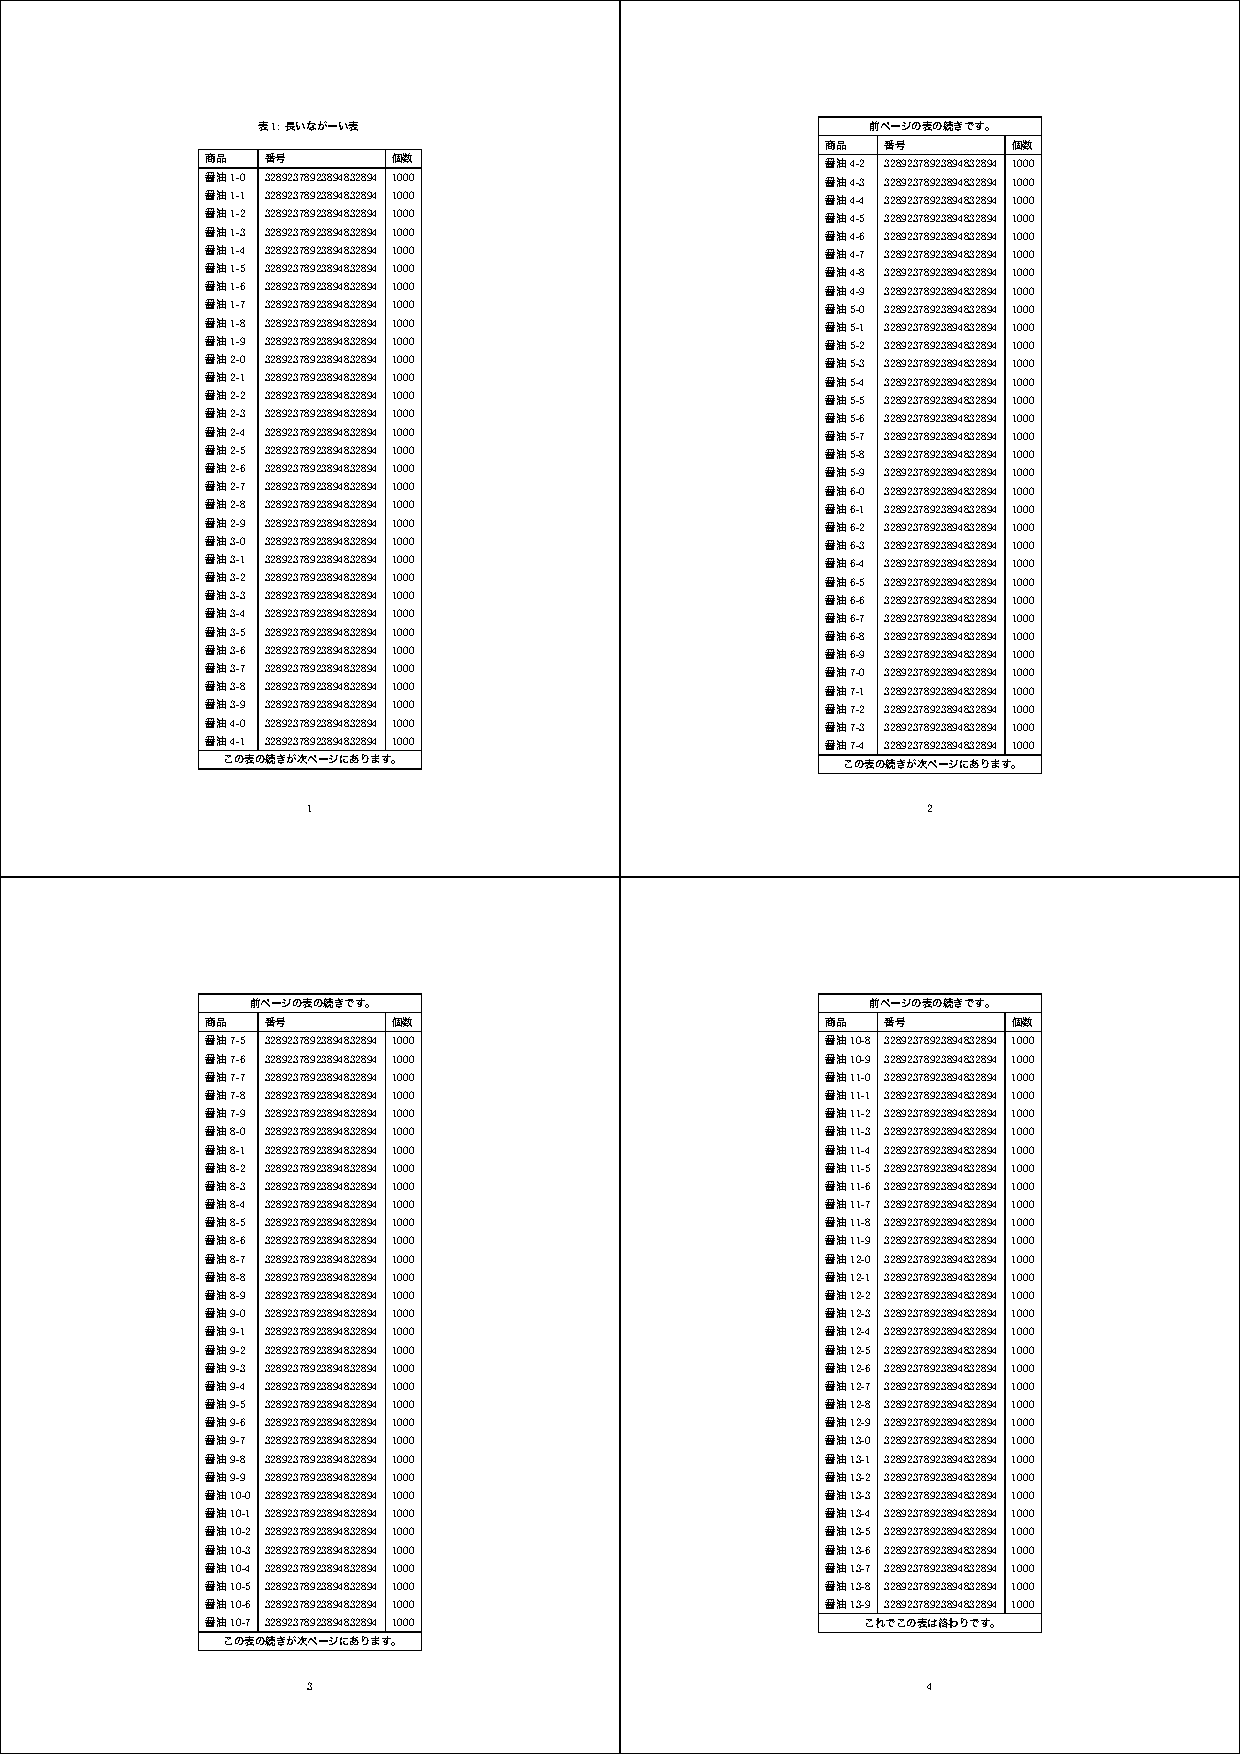
\includegraphics[width=\fullwidth]{longtable}%
 \caption{\Y{longtable}の使用例の出力結果}\figlab{longtable}%
\end{figure}

%\end{comment} 

\subsection{表の幅の指定\zdash\Y{tabularx}}\seclab{tabularx}
\LaTeXe の \E{array}/\E{tabular} 環境では列の幅を直接指定できる
列指定 `\str p\param{幅}' が用意されていますが,原稿を執筆している段階
ではその幅を決定できない事がしばしばあります.自動的にその幅を求め
てくれるような環境があれば便利です.そこで \Person{David}{Carlisle}の作成
した \Y{tabularx} パッケージを用いる事で \E{tabularx} 環境が使えます.
\begin{usage}
\begin{tabularx}{$\<幅>$}{$\<列指定>$}
$\<表を構成する要素>$ 
\end{tabularx} 
\end{usage}
%\begin{Syntax}
%\cmd{begin}\verb|{tabularx}|\param{幅}\param{列指定}\\
%\va{表を構成する要素}\\
%\cmd{end}\verb|{tabularx}| 
%\end{Syntax}
具体例を以下に示します.


\begin{intext}
\documentclass[a4j,10pt,papersize]{jsarticle}
\usepackage{tabularx}
\makeatletter
\def\hoge{\@tempcnta=\z@ \@whilenum \@tempcnta<10\do{%
   ○○○○\advance\@tempcnta\@ne}。}
\makeatother
\begin{document}
\hoge%
 \begin{center}
  \begin{tabularx}{\linewidth}{|X|X|X|}
   \hline
   \hoge & \hoge & \hoge \\
   \hline
  \end{tabularx}
 \end{center}
\hoge%
\begin{center}
 \begin{tabularx}{\linewidth}{|r|l|X|l|X|}
  \hline
  商品   & 値段 & 説明  & 型番 & 補足事項 \\
  \hline
  鍋     &  500 & \hoge & 59A  & \hoge    \\
  \hline
  やかん &  300 & \hoge & 9JA  & \hoge    \\
  \hline
 \end{tabularx}
\end{center}
\hoge%
\end{document}
\end{intext}

上記の入力の出力例は\figref{tabularx}となります.

\begin{figure}[htbp]
 \begin{center}
\makeatletter
\def\hoge{\@tempcnta=\z@ \@whilenum \@tempcnta<10\do{%
   ○○○○\advance\@tempcnta\@ne}。}%
\makeatother
  \begin{tabularx}{\linewidth}{|X|X|X|}
   \hline
   \hoge & \hoge & \hoge \\
   \hline
  \end{tabularx}\par\vskip1em
 \begin{tabularx}{\linewidth}{|r|l|X|l|X|}
  \hline
  商品   & 値段 & 説明  & 型番 & 補足事項 \\
  \hline
  鍋     &  500 & \hoge & 59A  & \hoge    \\
  \hline
  やかん &  300 & \hoge & 9JA  & \hoge    \\
  \hline
 \end{tabularx}
\caption{\Y{tabularx}使用例の出力結果\label{fig:tabularx}}
\end{center}
\end{figure}
%
\E{tabularx} 環境において列指定 `X' が新たに使えるようになっています.
\E{tabularx} 環境は組むべき表の幅を知る必要があります.`X' が複数の場合は
それぞれの列の幅は均等な長さになります.

%\subsection{表作成支援ツール}
%
%{\LaTeX}でゼロから表を組むのは初心者には
%辛いかもしれません.GUIベースの
%プログラムで表を作成し,それを{\LaTeX}の
%\env{tabular}環境の記述に変換するツールを
%使うと良いでしょう.Microsoftの\Prog{Excel}
%を使っている場合は\Hito{浦壁}{厚郎}の
%\Prog{Excel2tabular}\footnote\webEtoT
%などがありますので参考にしてください.これらの
%プログラムは{Microsoft}の\Prog{Excel}で作成さ
%れた表を{\LaTeX}のソースに変換します.
%
%MicrosoftのExcelではなく{OpenOffice.org}の
%\Prog{Calc}を使っているならば\Hito{阿部}{昌平}の
%\Prog[calc2latex]{Calc2\LaTeX}\footnote \webCtoL
%というものもあります.
%これを使えばCalcで作成した表を\env{tabular}環境に
%変換し,表として{\LaTeX}に貼り付ける事ができます.
%
%最近では直接 \LaTeX から \Prog{Excel} ファイルを読み込める
%\Person{Hans-Peter}{Doerr}による \Y{exceltex} パッケージが
%あります\footnote{\webExceltex}.
%\Prog{Perl}スクリプトを仲介する事で指定したセルやシートを読み込む事がで
%きます.

% end of table


\section{ヘッダ}

\subsection{日本語のヘッダを縦書きにする}

文章幅に対して表の横幅が長過ぎる場合に有効.
\begin{inout}
\begin{center}
  \newcommand*\TM[1]{\hbox{\tate#1}}
  \begin{tabular}{lccc}
   \hline
   属性\名前 &\TM{水銀灯} & \TM{金糸雀}& \TM{真紅}\\
   \hline 
   跳躍力   & 8& 5& 7\\  
   持久力   & 9& 6& 8\\  
   運の良さ & 8& 2& 7\\  
   \hline
  \end{tabular}
\end{center}
\end{inout}

\subsection{欧文のヘッダを縦方向に組む}

\begin{inout}
\begin{center}
 \newcommand*\TM[1]{\rotatebox{70}{#1}}
 \begin{tabular}{*4l}
  \hline
  \TM{Property$\backslash$Name}  &
  \TM{Mercury Lampe} & \TM{Kanarienvogel}& \TM{Reiner Rubin}\\
  \hline
  Weapon            & saber  & violin    & walking stick\\  
  Artificial Spirit & Meimei & Pizzicato & Hollie\\  
  Medium            & Megu   & Jun       & Mitsu\\  
  % 1st season において Mercury Lampe の Medium は存在しなかった.
  \hline
 \end{tabular}
\end{center}
\end{inout}

\subsection{\sty{array}パッケージ}
\sty{colortbl}
\sty{tabularx}
\sty{dcolumn}
\sty{delarray}
全てが \sty{array}パッケージを内部で自動的に読み込んでいます.
{\arrayrulewidth=3pt\begin{tabular}{|c||c|c|}
 \hline
 a& b& c\\
 \hline\hline
 d& e& f\\
 \hline
 g& h& i\\
 \hline
\end{tabular}}


\subsection{表の左上・右上に斜線を引く}

\Y{slashbox}

\begin{usage}
\usepackage{epic,eepic,slashbox}
\backslashbox{$\<左のテキスト>$}{$\<右のテキスト>$}
\slashbox{$\<左のテキスト>$}{$\<右のテキスト>$}
\end{usage}

%\begin{inout}
%\begin{center}
%\begin{tabular}[t]{|c|c|c|}
% \hline
% \backslashbox{氏名}{属性} & 跳躍力 [m] & 握力(左/右) [kg]\\
% \hline
%渡辺徹   & 1.5& 60.2/53.4\\ 
%佐藤利雄 & 2.2& 45.2/50.5\\ 
% \hline
%\end{tabular} 
%\end{center} 
%\end{inout}

\begin{usage}
 \usepackage{graphicx,eclarith,emathT}
\end{usage}

\begin{table}
\begin{center}
\caption{時間割}
\begin{Hyou}{|c||c|c||c|}\hline
\sya(6zw)[r]<\Hyoumidasi{時限}{曜日}> & 月 & 火 & \sya(7zw)[n]<\Hyoumidasi{時限}{曜日}> \\
\hline \hline
 1 & 体操 & 遊技 &1\\ \hline
 2 & 算数 & 国語 &2\\ \hline
\end{Hyou}
\end{center}
\end{table}

%\begin{table}[thbp]
% \begin{center}
% \caption{時間割}
% \begin{tabular}{|c||c|c||c|}\hline
% \backslashbox{時限}{曜日}& \makebox[3em]{月}& \makebox[3em]{火}&\slashbox{曜日}{時限} \\
% \hline \hline
% 1 & 体操 & 遊技 &1\\ \hline
% 2 & 算数 & 国語 &2\\ \hline
% \end{tabular}
% \end{center}
%\end{table}



